% Options for packages loaded elsewhere
\PassOptionsToPackage{unicode}{hyperref}
\PassOptionsToPackage{hyphens}{url}
\PassOptionsToPackage{dvipsnames,svgnames,x11names}{xcolor}
%
\documentclass[
  letterpaper,
  DIV=11]{scrartcl}

\usepackage{amsmath,amssymb}
\usepackage{iftex}
\ifPDFTeX
  \usepackage[T1]{fontenc}
  \usepackage[utf8]{inputenc}
  \usepackage{textcomp} % provide euro and other symbols
\else % if luatex or xetex
  \usepackage{unicode-math}
  \defaultfontfeatures{Scale=MatchLowercase}
  \defaultfontfeatures[\rmfamily]{Ligatures=TeX,Scale=1}
\fi
\usepackage{lmodern}
\ifPDFTeX\else  
    % xetex/luatex font selection
\fi
% Use upquote if available, for straight quotes in verbatim environments
\IfFileExists{upquote.sty}{\usepackage{upquote}}{}
\IfFileExists{microtype.sty}{% use microtype if available
  \usepackage[]{microtype}
  \UseMicrotypeSet[protrusion]{basicmath} % disable protrusion for tt fonts
}{}
\makeatletter
\@ifundefined{KOMAClassName}{% if non-KOMA class
  \IfFileExists{parskip.sty}{%
    \usepackage{parskip}
  }{% else
    \setlength{\parindent}{0pt}
    \setlength{\parskip}{6pt plus 2pt minus 1pt}}
}{% if KOMA class
  \KOMAoptions{parskip=half}}
\makeatother
\usepackage{xcolor}
\usepackage{soul}
\setlength{\emergencystretch}{3em} % prevent overfull lines
\setcounter{secnumdepth}{-\maxdimen} % remove section numbering
% Make \paragraph and \subparagraph free-standing
\ifx\paragraph\undefined\else
  \let\oldparagraph\paragraph
  \renewcommand{\paragraph}[1]{\oldparagraph{#1}\mbox{}}
\fi
\ifx\subparagraph\undefined\else
  \let\oldsubparagraph\subparagraph
  \renewcommand{\subparagraph}[1]{\oldsubparagraph{#1}\mbox{}}
\fi


\providecommand{\tightlist}{%
  \setlength{\itemsep}{0pt}\setlength{\parskip}{0pt}}\usepackage{longtable,booktabs,array}
\usepackage{calc} % for calculating minipage widths
% Correct order of tables after \paragraph or \subparagraph
\usepackage{etoolbox}
\makeatletter
\patchcmd\longtable{\par}{\if@noskipsec\mbox{}\fi\par}{}{}
\makeatother
% Allow footnotes in longtable head/foot
\IfFileExists{footnotehyper.sty}{\usepackage{footnotehyper}}{\usepackage{footnote}}
\makesavenoteenv{longtable}
\usepackage{graphicx}
\makeatletter
\def\maxwidth{\ifdim\Gin@nat@width>\linewidth\linewidth\else\Gin@nat@width\fi}
\def\maxheight{\ifdim\Gin@nat@height>\textheight\textheight\else\Gin@nat@height\fi}
\makeatother
% Scale images if necessary, so that they will not overflow the page
% margins by default, and it is still possible to overwrite the defaults
% using explicit options in \includegraphics[width, height, ...]{}
\setkeys{Gin}{width=\maxwidth,height=\maxheight,keepaspectratio}
% Set default figure placement to htbp
\makeatletter
\def\fps@figure{htbp}
\makeatother

\KOMAoption{captions}{tableheading}
\makeatletter
\@ifpackageloaded{tcolorbox}{}{\usepackage[skins,breakable]{tcolorbox}}
\@ifpackageloaded{fontawesome5}{}{\usepackage{fontawesome5}}
\definecolor{quarto-callout-color}{HTML}{909090}
\definecolor{quarto-callout-note-color}{HTML}{0758E5}
\definecolor{quarto-callout-important-color}{HTML}{CC1914}
\definecolor{quarto-callout-warning-color}{HTML}{EB9113}
\definecolor{quarto-callout-tip-color}{HTML}{00A047}
\definecolor{quarto-callout-caution-color}{HTML}{FC5300}
\definecolor{quarto-callout-color-frame}{HTML}{acacac}
\definecolor{quarto-callout-note-color-frame}{HTML}{4582ec}
\definecolor{quarto-callout-important-color-frame}{HTML}{d9534f}
\definecolor{quarto-callout-warning-color-frame}{HTML}{f0ad4e}
\definecolor{quarto-callout-tip-color-frame}{HTML}{02b875}
\definecolor{quarto-callout-caution-color-frame}{HTML}{fd7e14}
\makeatother
\makeatletter
\makeatother
\makeatletter
\makeatother
\makeatletter
\@ifpackageloaded{caption}{}{\usepackage{caption}}
\AtBeginDocument{%
\ifdefined\contentsname
  \renewcommand*\contentsname{Inhaltsverzeichnis}
\else
  \newcommand\contentsname{Inhaltsverzeichnis}
\fi
\ifdefined\listfigurename
  \renewcommand*\listfigurename{Abbildungsverzeichnis}
\else
  \newcommand\listfigurename{Abbildungsverzeichnis}
\fi
\ifdefined\listtablename
  \renewcommand*\listtablename{Tabellenverzeichnis}
\else
  \newcommand\listtablename{Tabellenverzeichnis}
\fi
\ifdefined\figurename
  \renewcommand*\figurename{Abbildung}
\else
  \newcommand\figurename{Abbildung}
\fi
\ifdefined\tablename
  \renewcommand*\tablename{Tabelle}
\else
  \newcommand\tablename{Tabelle}
\fi
}
\@ifpackageloaded{float}{}{\usepackage{float}}
\floatstyle{ruled}
\@ifundefined{c@chapter}{\newfloat{codelisting}{h}{lop}}{\newfloat{codelisting}{h}{lop}[chapter]}
\floatname{codelisting}{Listing}
\newcommand*\listoflistings{\listof{codelisting}{Listingverzeichnis}}
\makeatother
\makeatletter
\@ifpackageloaded{caption}{}{\usepackage{caption}}
\@ifpackageloaded{subcaption}{}{\usepackage{subcaption}}
\makeatother
\makeatletter
\@ifpackageloaded{tcolorbox}{}{\usepackage[skins,breakable]{tcolorbox}}
\makeatother
\makeatletter
\@ifundefined{shadecolor}{\definecolor{shadecolor}{rgb}{.97, .97, .97}}
\makeatother
\makeatletter
\makeatother
\makeatletter
\makeatother
\ifLuaTeX
\usepackage[bidi=basic]{babel}
\else
\usepackage[bidi=default]{babel}
\fi
\babelprovide[main,import]{ngerman}
% get rid of language-specific shorthands (see #6817):
\let\LanguageShortHands\languageshorthands
\def\languageshorthands#1{}
\ifLuaTeX
  \usepackage{selnolig}  % disable illegal ligatures
\fi
\IfFileExists{bookmark.sty}{\usepackage{bookmark}}{\usepackage{hyperref}}
\IfFileExists{xurl.sty}{\usepackage{xurl}}{} % add URL line breaks if available
\urlstyle{same} % disable monospaced font for URLs
\hypersetup{
  pdftitle={Empfehlungen der Medienleitlinie},
  pdflang={de},
  colorlinks=true,
  linkcolor={blue},
  filecolor={Maroon},
  citecolor={Blue},
  urlcolor={Blue},
  pdfcreator={LaTeX via pandoc}}

\title{Empfehlungen der Medienleitlinie}
\author{}
\date{}

\begin{document}
\maketitle
\ifdefined\Shaded\renewenvironment{Shaded}{\begin{tcolorbox}[frame hidden, borderline west={3pt}{0pt}{shadecolor}, interior hidden, breakable, boxrule=0pt, enhanced, sharp corners]}{\end{tcolorbox}}\fi

\renewcommand*\contentsname{Inhaltsverzeichnis}
{
\hypersetup{linkcolor=}
\setcounter{tocdepth}{3}
\tableofcontents
}
\begin{tcolorbox}[enhanced jigsaw, left=2mm, leftrule=.75mm, colframe=quarto-callout-note-color-frame, rightrule=.15mm, colback=white, arc=.35mm, opacityback=0, breakable, bottomrule=.15mm, toprule=.15mm]
\begin{minipage}[t]{5.5mm}
\textcolor{quarto-callout-note-color}{\faInfo}
\end{minipage}%
\begin{minipage}[t]{\textwidth - 5.5mm}

Die folgenden Empfehlungen sind entnommen aus:

Deutsche Gesellschaft für Kinder- und Jugendmedizin e.V. DGKJ.
SK2-Leitlinie: \textbf{Leitlinie zur Prävention dysregulierten
Bildschirmmediengebrauchs in der Kindheit und Jugend}. 1. Auflage 2023.
AWMF-Register Nr. 027-075. Verfügbar:
\url{https://register.awmf.org/de/leitlinien/detail/027-075}, Zugriff am
02.09.2023

\end{minipage}%
\end{tcolorbox}

\hypertarget{sec-die-wichtigsten-empfehlungen-auf-einen-blick}{%
\subsection*{Die wichtigsten Empfehlungen auf einen
Blick}\label{sec-die-wichtigsten-empfehlungen-auf-einen-blick}}
\addcontentsline{toc}{subsection}{Die wichtigsten Empfehlungen auf einen
Blick}

Für Kinder und Jugendliche gilt im Allgemeinen: Je weniger
Bildschirmzeit, desto besser.

Eltern sollen informiert und unterstützt werden,\ldots{}

\ldots{} Kinder unter 3 Jahren von jeglicher passiven und aktiven
Nutzung von Bildschirmmedien fernzuhalten.

\ldots{} falls sie ihre Kinder im Alter von 3 bis 6 Jahren an die
Nutzung von Bildschirmmedien heranführen möchten, dies höchstens 30
Minuten an einzelnen Tagen zu gestatten, und nicht ohne Anwesenheit der
Eltern.

\ldots{} Kindern im Alter von 6 bis 9 Jahren die freizeitliche Nutzung
von Bildschirmmedien höchstens 30 bis 45 Minuten an einzelnen Tagen zu
gestatten.

\ldots{} Kindern unter 9 Jahren keine eigene Spielkonsole zugänglich zu
machen.

\ldots{} Bildschirmmedien nicht zur Belohnung, Bestrafung oder
Beruhigung einzusetzen.

\ldots{} während des Essens, insbesondere der gemeinsamen Mahlzeiten,
keine Bildschirmmedien zu nutzen und bei der Nutzung von
Bildschirmmedien nicht zu essen.

\ldots{} sich für die digitalen Aktivitäten ihrer Kinder zu
interessieren und diese kritisch zu begleiten.

\ldots{} die Gefahr einer problematischen Nutzung von Onlinemedien zu
beachten (einschließlich evtl. Suchtentwicklung), die Bildschirmnutzung
Heranwachsender regelmäßig, gegebenenfalls gemeinsam, zu reflektieren
sowie im Zweifel anerkannte Tests zu nutzen und im Bedarfsfall
professionelle Hilfe zu suchen.

Eltern und Geschwister sollen informiert und unterstützt werden,\ldots{}

\ldots{} sich ihrer eigenen Vorbildfunktion für die aktive und passive
Bildschirmnutzung bewusst zu sein.

\ldots{} in Gegenwart von jüngeren Familienmitgliedern auf die Nutzung
von Bildschirmmedien zu verzichten.

Eltern und Lehrer*innen sollen informiert und unterstützt werden, auf
digitalen Fernunterricht wann immer möglich zu verzichten.

\hypertarget{allgemeine-empfehlungen-siehe-auch-altersspezifische-empfehlungen}{%
\subsection{\texorpdfstring{Allgemeine Empfehlungen (siehe auch
\protect\hyperlink{altersspezifische-empfehlungen}{altersspezifische
Empfehlungen})}{Allgemeine Empfehlungen (siehe auch altersspezifische Empfehlungen)}}\label{allgemeine-empfehlungen-siehe-auch-altersspezifische-empfehlungen}}

\begin{longtable}[]{@{}
  >{\raggedright\arraybackslash}p{(\columnwidth - 2\tabcolsep) * \real{0.0191}}
  >{\raggedright\arraybackslash}p{(\columnwidth - 2\tabcolsep) * \real{0.9809}}@{}}
\toprule\noalign{}
\begin{minipage}[b]{\linewidth}\raggedright
\end{minipage} & \begin{minipage}[b]{\linewidth}\raggedright
\textbf{Eltern sollen informiert und unterstützt werden, \ldots{}}
\end{minipage} \\
\midrule\noalign{}
\endhead
\bottomrule\noalign{}
\endlastfoot
1. & \ldots{} dass ihre Kinder leitliniengemäß, altersabhängig
ausreichend körperliche Freizeitaktivitäten ausüben. \\
2. & \ldots{} medienfreie Zeiträume zu schaffen, in denen die Familie
gemeinsame Aktivitäten unternimmt. \\
3. & ... während des Essens, insbesondere der gemeinsamen Mahlzeiten,
keine Bildschirmmedien zu nutzen und bei der Nutzung von
Bildschirmmedien nicht zu essen. \\
4. & ... dass sich während des Schlafens keine mobilen Bildschirmmedien
im Zimmer befinden, möglichst auch keine stationären Bildschirmmedien,
wie TV-Geräte oder Computer. \\
5. & \ldots{} dass ihre Kinder keine Bildschirmmedien in der letzten
Stunde vor dem Schlafengehen nutzen. \\
6. & \ldots{} dass ihre Kinder einen adäquaten, von aktiver wie passiver
Mediennutzung ungestörten Schlaf (je nach Alter des Kindes) bekommen. \\
7. & \ldots{} die Zeiten morgens vor Schule und Kindergarten möglichst
ohne Bildschirmmedien zu gestalten. \\
8. & \ldots{} Bildschirmmedien nicht zur Belohnung, Bestrafung oder
Beruhigung einzusetzen. \\
9. & ... ihre Kinder hinsichtlich einer vielfältigen Kommunikation, auch
ohne elektronische Geräte, zu unterstützen und anzuleiten (persönliche
Konversation, Telefonate, Briefe etc.). \\
10. & ... klare Regeln bezüglich der Nutzungsdauer von Bildschirmmedien
gemeinsam schriftlich zu vereinbaren und gemeinsam umzusetzen. Bewusste
Ausnahmen kann es geben, diese sollten ebenfalls schriftlich
festgehalten werden. \\
11. & \ldots{} die Bildschirmzeit verschieden alter Kinder in derselben
Familie entsprechend unterschiedlich zu gestalten. \\
12. & \ldots{} vor der Einführung mobiler Geräte mit Internetfähigkeit
einen „Handynutzungsvertrag'' unter Einbeziehung der Kinder zu
vereinbaren, unter Berücksichtigung der haftungsrechtlichen Situation,
soweit die Eltern die Besitzer des Gerätes sind und es dem Kind zur
Nutzung überlassen. \\
13. & \ldots{} Internet-Zugangssicherungen zu kennen und diese
einzusetzen, um Kinder vor altersunangemessenen Inhalten sowie
übermäßigem Konsum zu schützen. \\
14. & \ldots{} dass Ablenkungen während der Hausaufgaben durch
Bildschirmmedien vermieden und diese nur zweckgebunden eingesetzt
werden. \\
15. & \ldots{} sich an Altersempfehlungen von Medien zu orientieren und
diese nicht zu unterschreiten. Hierbei ist das Entwicklungsalter zu
berücksichtigen und im Zweifelsfall ein höheres Einstiegsalter zu
wählen. \\
16. & \ldots{} die Gefahr einer problematische Nutzung von Onlinemedien
zu beachten (einschließlich evtl. Suchtentwicklung), die
Bildschirmnutzung Heranwachsender regelmäßig, gegebenenfalls gemeinsam,
zu reflektieren sowie im Zweifel anerkannte Selbsttests zu nutzen und im
Bedarfsfall professionelle Hilfe zu suchen. \\
17. & \ldots{} beim Bewegtbildkonsum werbefreien Angeboten den Vorzug zu
geben und während etwaiger Werbepausen den Ton oder den gesamten
Bildschirm auszustellen. \\
18. & \ldots{} eigenständig für angemessene sexuelle Aufklärung ihrer
Kinder zu sorgen, bevor diese durch Mediennutzung mit sexuellen Inhalten
konfrontiert werden. \\
19. & \ldots{} mit anderen Bezugspersonen der Kinder neben den Eltern,
die bestehenden Regeln bezüglich der Nutzung von Bildschirmmedien
abzustimmen und zu besprechen, damit diese konsistent eingehalten werden
können. \\
20. & ... ein Netzwerk von Vertrauenspersonen aufzubauen, die für sich
und ihre Kinder als Anlaufstelle bei Schwierigkeiten dienen können. \\
21. & ... das Thema der Bildschirmmedien auch in Bildungseinrichtungen,
z.~B. als Themenschwerpunkt für Elternabende anzusprechen, um eine
konzertierte Aufklärung/Prävention mit den Bildungseinrichtungen und
innerhalb der jeweiligen Klassengemeinschaften umzusetzen. \\
22. & \ldots{} sich für die digitalen Aktivitäten ihrer Kinder zu
interessieren und diese kritisch zu begleiten. \\
23. & \ldots{} Bildschirmmedien bei Nichtbenutzung wegzuräumen, ggf. an
einem unzugänglichen und nicht sichtbaren Ort aufzubewahren („Aus den
Augen -- aus dem Sinn!{}``). \\
24. & \ldots{} möglichst auf Fernbedienungen und Sprachsteuerungen zu
verzichten und diese ihren Kindern unzugänglich zu machen. \\
\end{longtable}

\hypertarget{altersspezifische-empfehlungen}{%
\subsection{Altersspezifische
Empfehlungen}\label{altersspezifische-empfehlungen}}

Mit dem Älterwerden des Kindes ist der Übergang von einer direktiven hin
zu einer dialogischen Umsetzung der folgenden Empfehlungen angebracht.
In Einzelfällen müssen in Hinblick auf die vorgeschlagene Nutzungszeit
von Bildschirmmedien individuelle Maßstäbe angelegt werden. Dies gilt
insbesondere für eine Nutzung, die kreativen, edukativen und
selbstentwicklungsrelevanten Zwecken dient.

\begin{longtable}[]{@{}
  >{\raggedright\arraybackslash}p{(\columnwidth - 2\tabcolsep) * \real{0.0141}}
  >{\raggedright\arraybackslash}p{(\columnwidth - 2\tabcolsep) * \real{0.9859}}@{}}
\toprule\noalign{}
\begin{minipage}[b]{\linewidth}\raggedright
\end{minipage} & \begin{minipage}[b]{\linewidth}\raggedright
\textbf{Eltern sollen informiert und unterstützt werden, \ldots{}}
\end{minipage} \\
\midrule\noalign{}
\endhead
\bottomrule\noalign{}
\endlastfoot
& \ul{\textbf{0 bis 3 Jahre}} \\
25. & \ldots{} Kinder unter 3 Jahren von jeglicher passiven und aktiven
Nutzung von Bildschirmmedien fernzuhalten. \\
& \ul{\textbf{3 bis 6 Jahre}} \\
26. & ... falls sie ihre Kinder im Alter von 3 bis 6 Jahren an die
Nutzung von Bildschirmmedien heranführen möchten, dies höchstens 30
Minuten an einzelnen Tagen zu gestatten, und nicht ohne Anwesenheit der
Eltern. Dabei sollen sie auf qualitativ hochwertige Inhalte achten und
die Inhalte besprechen. Die Altersempfehlungen sollen eingehalten und
Inhalte im Vorfeld auf die Eignung für das eigene Kind hin geprüft
werden. \\
& \ul{\textbf{6 bis 9 Jahre}} \\
27. & ... Kindern im Alter von 6 bis 9 Jahren die freizeitliche Nutzung
von Bildschirmmedien höchstens 30 bis 45 Minuten an einzelnen Tagen zu
gestatten. Dabei sollen sie qualitativ hochwertige Inhalte, wann möglich
immer gemeinsam mit ihren Kindern nutzen, und diese im Nachhinein
besprechen. Die Altersempfehlungen sollen eingehalten und Inhalte im
Vorfeld auf die Eignung für das eigene Kind hin geprüft werden. \\
28. & \ldots{} Kindern unter 9 Jahren keinen freien Internetzugang zu
gewähren, auch nicht beaufsichtigt. \\
29. & ... Kindern unter 9 Jahren keine eigene Spielkonsole zugänglich zu
machen. \\
& \ul{\textbf{9 bis 12 Jahre}} \\
30. & ... Kindern im Alter von 9 bis 12 Jahren die freizeitliche Nutzung
von Bildschirmmedien höchstens 45 bis 60 Minuten täglich zu gestatten.
Dabei sollen sie qualitativ hochwertige Inhalte, wann möglich immer
gemeinsam mit ihren Kindern nutzen, und diese im Nachhinein besprechen.
Die Altersempfehlungen sollen eingehalten und Inhalte im Vorfeld auf die
Eignung für das eigene Kind hin geprüft werden. \\
31. & ... Kinder frühestens ab 9 Jahren, besser frühestens ab 12 Jahren,
ein eigenes Smartphone mit eingeschränktem Internetzugang zu
überlassen. \\
32. & ... Kindern im Alter von 9 bis 12 Jahren nur beaufsichtigten
Internetzugang zu gewähren. \\
& \ul{\textbf{12 bis 16 Jahre}} \\
33. & ... Jugendlichen im Alter von 12 bis 16 Jahren die freizeitliche
Nutzung von Bildschirmmedien von maximal 1-2 Stunden am Tag und bis
spätestens 21 Uhr zu ermöglichen. Die Altersempfehlungen sollen beachtet
und Inhalte zudem im Vorfeld auf die Eignung für das eigene Kind hin
geprüft werden. Heranwachsende sollen weiterhin inhaltlich begleitet
werden. \\
34. & ... regelmäßig mit den Jugendlichen Gespräche führen, um die
Medienzeit und Inhalte, auch im Verhältnis zu den eigenen Lebenszielen,
zu reflektieren. Jugendliche sollen dazu angeregt werden, selber zu
beobachten, wie sich Medienkonsum auf Konzentration, Sozialverhalten,
Fitness, Persönlichkeit, Schulnoten etc. auswirken. \\
35. & ... Jugendlichen im Alter von 12 bis 16 Jahren nur beschränkten
Internetzugang zu gewähren. \\
36. & \ldots{} im Falle einer übermäßigen Internetnutzung anerkannte
Selbsttests zu nutzen und im Bedarfsfall professionelle Hilfe zu
suchen. \\
& \ul{\textbf{16 bis 18 Jahre}} \\
37. & ... je nach Reifegrad die freizeitliche Nutzung von
Bildschirmmedien durch Regeln festzulegen (z.B. an einem Abend vor einer
Klausur); ein Orientierungswert kann 2 Stunden am Tag betragen. Die
Altersempfehlungen sollen beachtet werden. Eltern sollen begleitend zur
Seite stehen und regelmäßig Gespräche zur Reflektion führen. \\
38. & \ldots{} Jugendlichen ab 16 Jahren den uneingeschränkten
Internetzugang zu ermöglichen. Die Erfahrung zeigt, dass auch 16 bis
18-jährige es sehr schwer haben können, Bildschirmmedienkonsum auf ein
gesundes Maß zu begrenzen. Viele von ihnen bedürfen immer noch einer
intensiven Begleitung. \\
39. & \ldots{} im Falle einer übermäßigen Internetnutzung gemeinsam mit
dem Jugendlichen einen anerkannten medienbezogenen Selbsttest
durchzuführen und sich möglichst frühzeitig professionelle Hilfe zu
suchen. \\
\end{longtable}

\hypertarget{empfehlungen-fuxfcr-den-digitalen-fernunterricht}{%
\subsection{Empfehlungen für den digitalen
Fernunterricht}\label{empfehlungen-fuxfcr-den-digitalen-fernunterricht}}

\begin{longtable}[]{@{}
  >{\raggedright\arraybackslash}p{(\columnwidth - 2\tabcolsep) * \real{0.0214}}
  >{\raggedright\arraybackslash}p{(\columnwidth - 2\tabcolsep) * \real{0.9786}}@{}}
\toprule\noalign{}
\begin{minipage}[b]{\linewidth}\raggedright
\end{minipage} & \begin{minipage}[b]{\linewidth}\raggedright
\textbf{Eltern und Lehrer*innen sollen informiert und unterstützt
werden, \ldots{}}
\end{minipage} \\
\midrule\noalign{}
\endhead
\bottomrule\noalign{}
\endlastfoot
40. & \ldots{} auf digitalen Fernunterricht wann immer möglich zu
verzichten.

In der Grundschule (Primarstufe) soll digitaler Fernunterricht auf ein
Minimum reduziert werden. Stattdessen soll auf analoge Materialien mit
Lernaufgaben für Eltern und Kinder zurückgegriffen werden, die in beide
Richtungen auf dem Postweg oder in digitalisierter Form (z.~B.
Ausdrucken/Einscannen) versendet werden.

In der weiterführenden Schule (Sekundarstufe I+II) ist digitaler
Fernunterricht im geringen Umfang möglich, dabei sollen die Schüler
mehrheitlich analoge Medien zur Aufgabenbewältigung einsetzen. \\
41. & \ldots{} die Stundenpläne des Präsenzunterrichts nicht 1: 1 auf
digitalen Unterricht zu übertragen.

In der Grundschule (Primarstufe) soll digitaler Fernunterricht eine
Bildschirmzeit von 60 Minuten am Tag nicht überschreiten.

In der weiterführenden Schule (Sekundarstufe I+II) soll digitaler
Fernunterricht eine Bildschirmzeit von 120 Minuten am Tag nicht
überschreiten. \\
42. & \ldots{} ein salutogenetisches Unterrichtskonzept zu erstellen,
incl.~Bewegungsausgleich, Augenhygiene, Umgang mit Natur, Kunst sowie
Soziales. Kinder sollen viele Anregungen für bildschirmfreie Arbeiten
erhalten. Pausen sind in digitalem Fernunterricht regelmäßig und
vermehrt einzuhalten. \\
43. & \ldots{} die Kinder außerhalb von digitalem Unterricht zu
bildschirmfreien Eigenaktivitäten anzuregen. \\
44. & \ldots sicherzustellen, dass auch Geräte, die von Schulen für den
digitalen Fernunterricht zur Verfügung gestellt werden, eine
Zeitbegrenzung und Filtersoftware beinhalten, damit diese nicht über die
Unterrichtszeit hinaus und nicht für entwicklungs-beeinträchtigende
Inhalte verwendet werden können. \\
45. & \ldots{} falls digitaler Fernunterricht erwogen oder z.~B. aus
pandemischen Gründen notwendig ist, sollen alle Möglichkeiten des
Unterrichtes oder der Förderung in Präsenz genutzt werden. \\
46. & \ldots{} sich der Gefahr von problematischer Mediennutzung bei den
Schüler*innen bewusst zu sein und geeignete Maßnahmen einzuleiten. \\
\end{longtable}

\hypertarget{empfehlungen-in-pandemiezeiten}{%
\subsection{Empfehlungen in
Pandemiezeiten}\label{empfehlungen-in-pandemiezeiten}}

\begin{longtable}[]{@{}
  >{\raggedright\arraybackslash}p{(\columnwidth - 2\tabcolsep) * \real{0.0303}}
  >{\raggedright\arraybackslash}p{(\columnwidth - 2\tabcolsep) * \real{0.9697}}@{}}
\toprule\noalign{}
\begin{minipage}[b]{\linewidth}\raggedright
\end{minipage} & \begin{minipage}[b]{\linewidth}\raggedright
\textbf{Eltern und Lehrer*innen sollen informiert und unterstützt
werden, \ldots{}}
\end{minipage} \\
\midrule\noalign{}
\endhead
\bottomrule\noalign{}
\endlastfoot
47. & ... in Pandemiezeiten \emph{vorrübergehende} Sonderregelungen für
die Nutzung von Bildschirmmedien für die Familie zu erstellen. \\
48. & ... während der Pandemie vermehrt Aktivitäten in der Natur, im
sozialen Nahraum und im kreativen Bereich zu ermöglichen. \\
49. & \ldots{} in und nach Pandemiezeiten gesundheitsfördernde,
ressourcen- und resilienzfördernde Präventionsprogramme mit ihren
Kindern/Schülern gemeinsam durchführen, bzw. die Inhalte zu
vermitteln. \\
50. & \ldots{} am Ende von Pandemiezeiten die Nutzung von
Bildschirmmedien auf das vorpandemische Niveau zu reduzieren und bewusst
medienfreie Zeiträume zu etablieren. \\
\end{longtable}

\hypertarget{empfehlungen-fuxfcr-eltern-und-geschwister-als-vorbilder}{%
\subsection{Empfehlungen für Eltern und Geschwister als
Vorbilder}\label{empfehlungen-fuxfcr-eltern-und-geschwister-als-vorbilder}}

\begin{longtable}[]{@{}
  >{\raggedright\arraybackslash}p{(\columnwidth - 2\tabcolsep) * \real{0.0190}}
  >{\raggedright\arraybackslash}p{(\columnwidth - 2\tabcolsep) * \real{0.9810}}@{}}
\toprule\noalign{}
\begin{minipage}[b]{\linewidth}\raggedright
\end{minipage} & \begin{minipage}[b]{\linewidth}\raggedright
\textbf{Eltern und Geschwister sollen informiert und unterstützt werden,
\ldots{}}
\end{minipage} \\
\midrule\noalign{}
\endhead
\bottomrule\noalign{}
\endlastfoot
51. & ... regelmäßig ihr eigenes Nutzungsverhalten zu reflektieren und
ggf. anzupassen. \\
52. & \ldots{} sich ihrer eigenen Vorbildfunktion für die aktive und
passive Bildschirmnutzung bewusst zu sein. \\
53. & \ldots{} in Gegenwart von jüngeren Familienmitgliedern auf die
Nutzung Bildschirmmedien zu verzichten. \\
54. & \ldots{} in Situationen, in denen in Gegenwart von Kindern und
Jugendlichen die Nutzung von Bildschirmmedien (z.~B. berufsbedingt) in
der Freizeit nicht vermeidbar ist, zuvor für alternative
Beschäftigungsmöglichkeiten zu sorgen. Den Kindern soll die
Notwendigkeit der Nutzung von Bildschirmmedien erklärt werden. \\
55. & \ldots{} im Falle einer übermäßigeren Internetnutzung einen
anerkannten medienbezogenen Selbsttest durchzuführen und sich ggf.
professionelle Hilfe zu suchen. \\
\end{longtable}

\hypertarget{vorgehen-im-falle-dysregulierter-bildschirmmediennutzung}{%
\subsection{Vorgehen im Falle dysregulierter
Bildschirmmediennutzung}\label{vorgehen-im-falle-dysregulierter-bildschirmmediennutzung}}

Abhängig von der Schwere der Dysregulation sowie des Alters des/der
Betroffenen muss individuell und fallbezogen von dem Therapeuten, der
primär angesprochen wird, entschieden werden, welche Hilfsangebote die
Familie braucht. Bei vielen Familien besteht basaler Beratungsbedarf und
ein Mangel an richtigen Informationen (z.~B. darüber, dass übermäßiger
Medienkonsum ungünstig für die Entwicklung von Kindern ist). Initial,
und damit auf einem „Informationslevel'', kann die jeweilig
angesprochene Person/Stelle zunächst mit entsprechenden Infomaterialien
und im Beratungsgespräch eventuelle Wissenslücken schließen, Fragen
beantworten, motivieren. Sind ausreichend Informationen vorhanden und
geht es um die gescheiterte Umsetzung derselben, ist ein
„Interventionslevel'' erreicht.

Zunächst müssen die Gründe verstanden werden, die dazu führen, dass
„wider besseres Wissens gehandelt wird''. Je nachdem, wie diese Gründe
sich darstellen, ergibt sich die Auswahl der dann auch fachkompetenten
Hilfe. Die eine Familie wird eine sozialpädagogische Fachkraft brauchen,
um zuhause die Umsetzung von Regeln zu ermöglichen, in der anderen
Familie mag eine größere psychosoziale Problematik der Anlass sein, dass
die Eltern oder z. B. das alleinerziehende Elternteil erschöpft und
daher nicht mehr in der Lage sind, konsequent zu handeln. Und in anderen
Fällen können Störungen der Impulskontrolle oder~ADHS die Ursache sein
und eine entsprechende Therapie notwendig werden.

Psychoedukation, Verhaltenstherapie und ggf. medikamentöse Therapie
müssen durch Fachleute in Spezialambulanzen, Beratungszentren oder
spezialisierten Praxen (Ärzt*innen, Psychotherapeut*innen,
Sozialtherapeuten, Pädagogen etc.) initiiert und oftmals auf längere
Zeit begleitet werden. In den seltensten Fällen reicht hier ein
einmaliges kurzes Beratungsgespräch aus. Die Problematik ist häufig
mehrdimensional, besteht bevor Beratung gewünscht wird, über mehrere
Jahre, und der dysregulierte oder gar suchthafte Medienkonsum ist nur
ein sichtbares Zeichen einer weit größeren Problematik.

Zur Definition „suchthafter Gebrauch'' sind hier die Kriterien der
„Internet Gaming Disorders'' in adaptierter Weise zu gebrauchen und auf
das Medienverhalten anzuwenden: Das revidierte DSM-5 (Diagnostisches und
Statistisches Manual Psychischer Störungen, fünfte Auflage), das von der
American Psychiatric Association herausgegeben wird, beinhaltet
„Internet Gaming Disorder'' als Forschungsdiagnose. Dazu müssen fünf der
folgenden Kriterien über 12 Monate erfüllt sein:

\begin{itemize}
\item
  andauernde Beschäftigung mit Internet- bzw. Online-Spielen
\item
  Entzugssymptome, wenn das Online-Spielen nicht zur Verfügung steht
\item
  Toleranzentwicklung mit dem Bedürfnis, zunehmend Zeit für
  Online-Spiele aufzubringen
\item
  erfolglose Versuche, die Teilnahme am Online-Spielen zu beenden
\item
  Verlust des Interesses an früheren Hobbies oder Aktivitäten als Folge
  des Online-Spielens
\item
  Andauerndes, exzessives Online-Spielen trotz des Wissens um die
  psychosozialen Probleme
\item
  Täuschen von Familienmitgliedern, Therapeuten oder anderen Personen in
  Bezug auf das wirkliche Ausmaß des Online-Spielens
\item
  Gebrauch der Online-Spiele, um aus negativen Emotionen (wie z.~B.
  Gefühlen von Hilflosigkeit, Schuld oder Ängstlichkeit) herauszukommen
  oder um diese zu lindern
\item
  Gefährdung oder Verlust von wichtigen Bekanntschaften, Beruf,
  Ausbildung oder Karriere-Möglichkeiten wegen des Online-Spielens
\end{itemize}

Bei Jugendlichen ist das unmittelbar anwendbar, für kleinere Kinder ist
es etwa so zu adaptieren:

\begin{itemize}
\item
  Beschäftigung mit Medien für eine erhebliche Zeit am Tag (ein
  Vielfaches der empfohlenen Zeit)
\item
  Entzugssymptome bei Medienverbot
\item
  Schwierigkeiten beim Beenden
\item
  Fixierung auf Medien
\item
  Mangelnde andere, altersadäquate Beschäftigungen sowie Beziehungen zu
  Gleichaltrigen
\item
  Medien einzige oder häufige Alternative, um negative Emotionen zu
  beenden
\end{itemize}

Verhaltenstherapie mit Förderung der Familienunterstützung und
Elterntrainings sind wirksame, aber auch aufwendige notwendige
Maßnahmen, in Einzelsituationen sind auch andere Therapien zu erwägen.
Zu beachten ist, dass das Kind/der/die Jugendliche zwar meist selbst
betroffen ist, aber nicht alleine therapiert werden kann. Das
Medienverhalten der ganzen Familie muss erfasst und meist auch bei allen
verändert werden, damit bei dem Kind/Jugendlichen überhaupt eine
grundlegende Änderung möglich ist (siehe Elternempfehlungen).

Oftmals ist ein strukturierter Tagesplan mit klar festgelegten und
altersgerecht angepassten Zeiten der erste Schritt. Klare Zeiten der
Mediennutzung müssen ritualisiert, erlernt und konsequent umgesetzt
werden. Für die Nicht-Nutzungszeiten wird empfohlen, die Geräte aus der
Reichweite der Kinder zu nehmen (Verwahrung im „Handybett'';
Wegschließen der Geräte, etc.). Auf Vermeidung des „passiven
Medienkonsums'', also des Mitschauens bei Eltern oder älteren
Geschwistern, auch im Rahmen des Unterrichtes ist zu achten. Häufig
benötigen die Familien Anleitung, Unterstützung und Begleitung, um
alternative Spielangebote machen zu können.

In einzelnen Fällen mit krisenhafter Zuspitzung, insbesondere bei
suchthaftem Gebrauch sind auch stationäre Aufenthalte notwendig. Vor
„radikalen Entzugskuren'' bei bestehendem suchthaftem Konsum ohne
therapeutische Begleitung im ambulanten Setting ist zu warnen, da die
sich ergebende Destabilisierung oft ambulant nicht abgefangen werden
kann. Das Handlungsschema in Abbildung~\ref{fig-handlungsschema} soll
bei dieser Beurteilung helfen.

\begin{figure}

{\centering 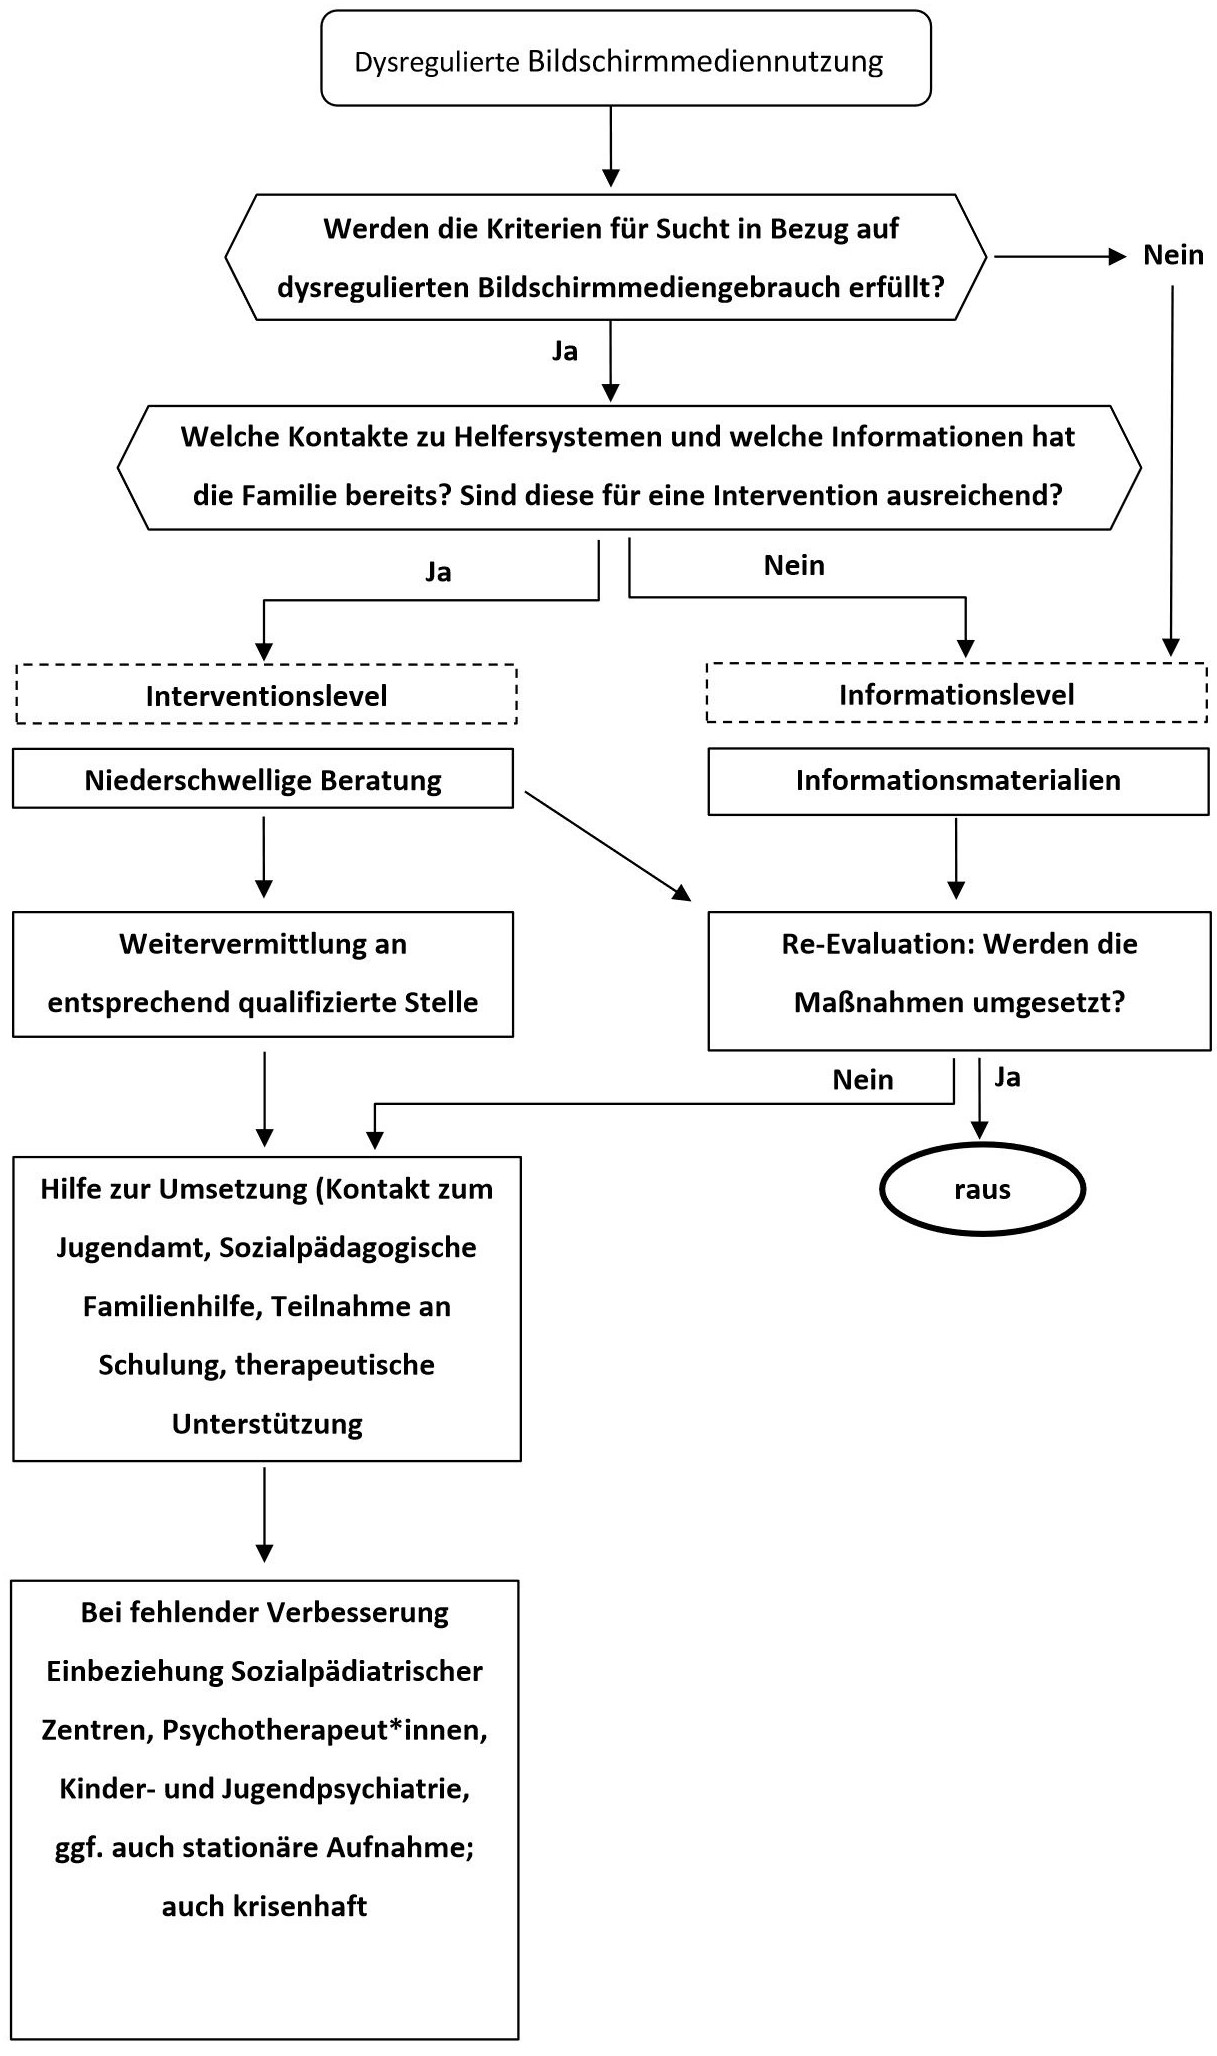
\includegraphics{images/handlungsschema.jpg}

}

\caption{\label{fig-handlungsschema}Handlungsschema zum Vorgehen im
Falle dysregulierter Bildschirmmediennutzung}

\end{figure}

\begin{longtable}[]{@{}
  >{\raggedright\arraybackslash}p{(\columnwidth - 2\tabcolsep) * \real{0.0239}}
  >{\raggedright\arraybackslash}p{(\columnwidth - 2\tabcolsep) * \real{0.9761}}@{}}
\toprule\noalign{}
\begin{minipage}[b]{\linewidth}\raggedright
\end{minipage} & \begin{minipage}[b]{\linewidth}\raggedright
\textbf{Empfehlungen zum Vorgehen im Falle dysregulierter
Bildschirmmediennutzung}
\end{minipage} \\
\midrule\noalign{}
\endhead
\bottomrule\noalign{}
\endlastfoot
56. & Als Basis soll die jeweilig beratende Person/Familie/Stelle
zunächst mit entsprechenden Informationsmaterialien ausgestattet werden.
Im anschließenden Beratungsgespräch sollen Wissenslücken geschlossen,
Fragen beantwortet und motiviert werden. \\
57. & Sind ausreichend Informationen vorhanden und geht es um die
gescheiterte Umsetzung derselben, sollen Psychoedukation,
Verhaltenstherapie und ggf. medikamentöse Therapie durch Fachleute
initiiert und auf längere Zeit begleitet werden. \\
58. & Das Medienverhalten der ganzen Familie soll erfasst und bei allen
ggf. verändert werden, damit bei den Kindern/Jugendlichen eine
grundlegende Änderung möglich ist. \\
59. & In einzelnen Fällen bei suchthaftem Mediengebrauch mit
krisenhafter Zuspitzung soll ein stationärer Aufenthalt indiziert
werden. \\
\end{longtable}



\end{document}
